\section{Date: 2026-10-12}
\noindent \textbf{Series ID: BOPBSVN} 

\noindent This series is titled Balance on Services (DISCONTINUED) and has a frequency of Quarterly. The units are Billions of Dollars and the seasonal adjustment is Not Seasonally Adjusted.The observation start date is 1960-01-01 and the observation end date is 2014-01-01.The popularity of this series is 1. \\ 

\noindent \textbf{Series ID: XRNCUSBZA618NRUG} 

\noindent This series is titled Exchange Rate (market+estimated) for Belize and has a frequency of Annual. The units are National Currency Units per US Dollar and the seasonal adjustment is Not Seasonally Adjusted.The observation start date is 1970-01-01 and the observation end date is 2023-01-01.The popularity of this series is 1. \\ 

\subsection{Raw Regression}
\noindent Regresses the two series against each other directly. A significant result here can come just as easily from both series sharing a long-run trend as from any real relationship.

\begin{center}
\begin{tabular}{lclc}
\toprule
\textbf{Dep. Variable:}       & value\_fred\_XRNCUSBZA618NRUG & \textbf{  R-squared:         } &     0.090   \\
\textbf{Model:}               &              OLS              & \textbf{  Adj. R-squared:    } &     0.069   \\
\textbf{Method:}              &         Least Squares         & \textbf{  F-statistic:       } &     4.246   \\
\textbf{Date:}                &        Mon, 12 Oct 2026       & \textbf{  Prob (F-statistic):} &   0.0454    \\
\textbf{Time:}                &            20:28:58           & \textbf{  Log-Likelihood:    } &    34.026   \\
\textbf{No. Observations:}    &                 45            & \textbf{  AIC:               } &    -64.05   \\
\textbf{Df Residuals:}        &                 43            & \textbf{  BIC:               } &    -60.44   \\
\textbf{Df Model:}            &                  1            & \textbf{                     } &             \\
\textbf{Covariance Type:}     &           nonrobust           & \textbf{                     } &             \\
\bottomrule
\end{tabular}
\begin{tabular}{lcccccc}
                              & \textbf{coef} & \textbf{std err} & \textbf{t} & \textbf{P$> |$t$|$} & \textbf{[0.025} & \textbf{0.975]}  \\
\midrule
\textbf{const}                &       1.9274  &        0.024     &    79.937  &         0.000        &        1.879    &        1.976     \\
\textbf{value\_fred\_BOPBSVN} &       0.0023  &        0.001     &     2.060  &         0.045        &     4.83e-05    &        0.004     \\
\bottomrule
\end{tabular}
\begin{tabular}{lclc}
\textbf{Omnibus:}       & 17.591 & \textbf{  Durbin-Watson:     } &    0.425  \\
\textbf{Prob(Omnibus):} &  0.000 & \textbf{  Jarque-Bera (JB):  } &   23.370  \\
\textbf{Skew:}          & -1.275 & \textbf{  Prob(JB):          } & 8.42e-06  \\
\textbf{Kurtosis:}      &  5.441 & \textbf{  Cond. No.          } &     30.5  \\
\bottomrule
\end{tabular}
%\caption{OLS Regression Results}
\end{center}

Notes: \newline
 [1] Standard Errors assume that the covariance matrix of the errors is correctly specified.

\begin{figure}
\centering
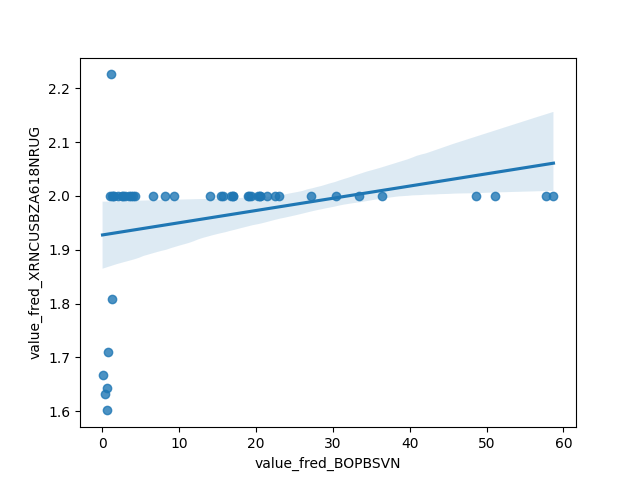
\includegraphics[scale = 0.9]{plots/plot_2026-10-12.png}
\caption{Raw Regression Plot for 2026-10-12}
\end{figure}
\newpage
\subsection{Detrended Regression}
\noindent Regresses the residuals of each series after removing its own linear time trend, so a shared trend can no longer drive the result on its own. A relationship that stays significant here is better evidence of a genuine link between the two series.

\begin{center}
\begin{tabular}{lclc}
\toprule
\textbf{Dep. Variable:}                  & value\_fred\_XRNCUSBZA618NRUG\_detrended & \textbf{  R-squared:         } &     0.123   \\
\textbf{Model:}                          &                   OLS                    & \textbf{  Adj. R-squared:    } &     0.103   \\
\textbf{Method:}                         &              Least Squares               & \textbf{  F-statistic:       } &     6.041   \\
\textbf{Date:}                           &             Mon, 12 Oct 2026             & \textbf{  Prob (F-statistic):} &   0.0181    \\
\textbf{Time:}                           &                 20:28:58                 & \textbf{  Log-Likelihood:    } &    41.263   \\
\textbf{No. Observations:}               &                      45                  & \textbf{  AIC:               } &    -78.53   \\
\textbf{Df Residuals:}                   &                      43                  & \textbf{  BIC:               } &    -74.91   \\
\textbf{Df Model:}                       &                       1                  & \textbf{                     } &             \\
\textbf{Covariance Type:}                &                nonrobust                 & \textbf{                     } &             \\
\bottomrule
\end{tabular}
\begin{tabular}{lcccccc}
                                         & \textbf{coef} & \textbf{std err} & \textbf{t} & \textbf{P$> |$t$|$} & \textbf{[0.025} & \textbf{0.975]}  \\
\midrule
\textbf{const}                           &    5.671e-15  &        0.015     &  3.84e-13  &         1.000        &       -0.030    &        0.030     \\
\textbf{value\_fred\_BOPBSVN\_detrended} &      -0.0050  &        0.002     &    -2.458  &         0.018        &       -0.009    &       -0.001     \\
\bottomrule
\end{tabular}
\begin{tabular}{lclc}
\textbf{Omnibus:}       &  8.915 & \textbf{  Durbin-Watson:     } &    0.588  \\
\textbf{Prob(Omnibus):} &  0.012 & \textbf{  Jarque-Bera (JB):  } &   16.952  \\
\textbf{Skew:}          &  0.296 & \textbf{  Prob(JB):          } & 0.000208  \\
\textbf{Kurtosis:}      &  5.948 & \textbf{  Cond. No.          } &     7.28  \\
\bottomrule
\end{tabular}
%\caption{OLS Regression Results}
\end{center}

Notes: \newline
 [1] Standard Errors assume that the covariance matrix of the errors is correctly specified.

\begin{figure}
\centering
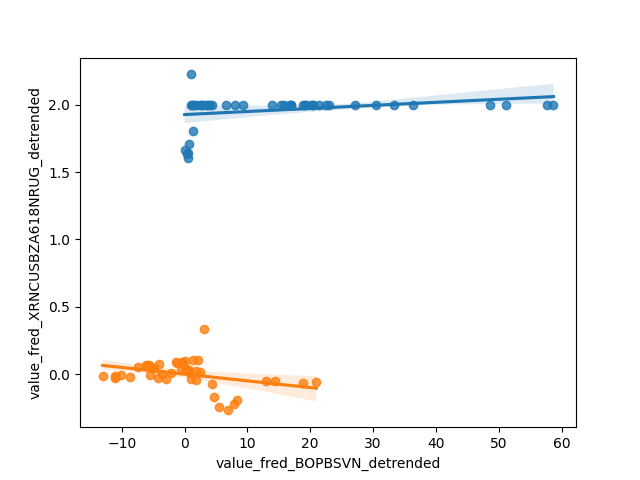
\includegraphics[scale = 0.9]{plots/plot_2026-10-12_detrended.png}
\caption{Detrended Regression Plot for 2026-10-12}
\end{figure}
\newpage
